\chapter{Perancangan}
\label{chap:perancangan}

\section{Rancangan Antarmuka}
Peracangan antarmuka dilakukan dengan langsung menggunakan HTML untuk mempercepat pengembangan aplikasi. Bootstrap\footnote{https://getbootstrap.com/} digunakan untuk mempercepat \textit{styling} pada HTML. Perancangan antarmuka tersebut dibagi menjadi tiga bagian besar berdasarkan analisa pengguna yang telah dilakukan pada bab sebelumnya.

\subsection{Rancangan Antarmuka untuk Peserta}


\subsection{Rancangan Antarmuka untuk Admin}


\subsection{Rancangan Antarmuka untuk Dosen Pengawas}

    % Jelasin kalo ini buat di proyektor

\section{Perancangan Sistem Backend}
    Sesuai dengan perannya, sistem backend akan bertanggung jawab menangani bagian-bagian yang hanya 
    ditangani pada sisi peladen. Tanggung jawab tersebut mulai dari melakukan pengolahan data,
    pengelolaan basis data, serta menyediakan API yang digunakan oleh sistem frontend untuk
    berkomunikasi.
    
    Pada bagian ini akan dijelaskan perancangan sistem untuk subsistem backend. Penjelasan tersebut
    dimulai dari pembahasan perancangan basis data, perancangan REST API 
    serta desain kelas dari subsistem ini.
    
\subsection{Racangan Basis Data}
    \begin{sidewaysfigure}
        \centering
        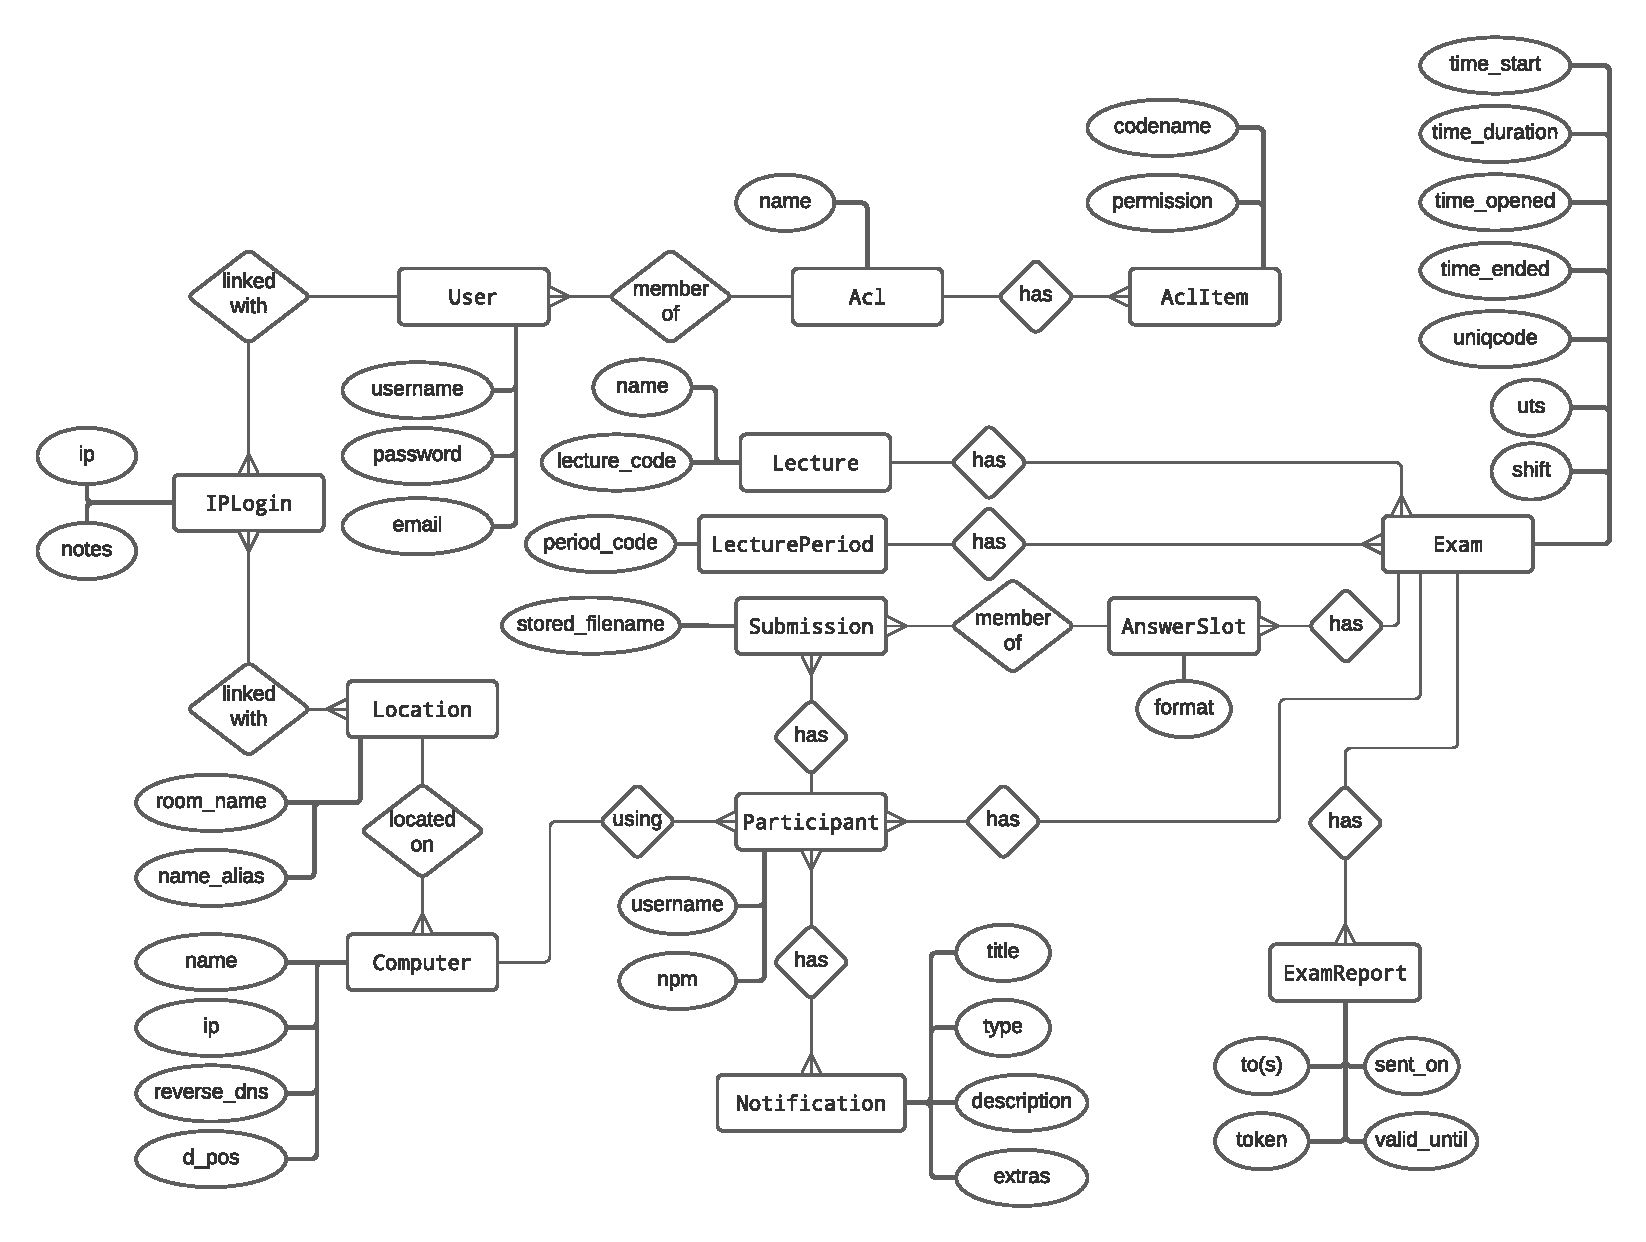
\includegraphics[width=1\paperwidth]{Gambar/erd-rev-b.pdf}
        \caption{Diagram \textit{ERD} untuk sistem aplikasi yang baru.}
        \label{fig:erd_overview}
    \end{sidewaysfigure}
    
    Perancangan basis data dimulai dengan merumuskan entitas yang dibutuhkan dan relasinya
    dengan entitas lainnya. Rumusan tersebut direpresentasikan dalam bentuk diagram relasi
    entitas atau ERD. Diagram ERD untuk aplikasi ini dapat dilihat pada Gambar \ref{fig:erd_overview}.
    Berdasarkan kebutuhan yang dianalisis pada bab sebelumnya, sistem membutuhkan empat belas
    entitas yang bertanggung jawab untuk merepresentasikan struktur data yang digunakan.
    Setiap entitas yang dibuat akan dibuat ulang representasinya dalam bentuk kelas pada
    sistem PHP dengan harapan membantu penanganan dan perancangan sistem REST API.
    
    Pembahasan akan dilanjutkan dengan menjelaskan satu per satu entitas yang ditunjukan
    pada diagram ERD. Pembahasan akan dimulai dengan entitas yang penulis kategorikan sebagai
    esensial untuk sistem terlebih dahulu, lalu dilanjutkan dengan entitas yang muncul dari
    analisis dari bab sebelumnya.
    
\subsubsection{User}
    % TODO: Figure mini user?.
    Entitas \texttt{User} merepresentasikan pengguna aplikasi. Entitas ini akan menyimpan informasi
    khusus seperti nama pengguna (\texttt{username}), kata sandi (\texttt{password}) dan email.
    Kolom \texttt{password} pada entitas ini akan di\textit{hash} menggunakan algoritma Blowfish
    dengan bantuan \textit{library} dari PHP dengan alasan keamanan.
    
    Entitas ini dinilai esensial karena entitas ini digunakan untuk melakukan otentikasi
    menuju panel admin. Entitas ini akan memiliki perlakuan khusus pada saat data
    dari entitas ini ditransmisikan ke sistem frontend. Otentikasi ini penting untuk
    mengkhususkan peran dari setiap pengguna.

\subsubsection{ACL dan ACLItem}
    \begin{figure}[H]
        \centering
        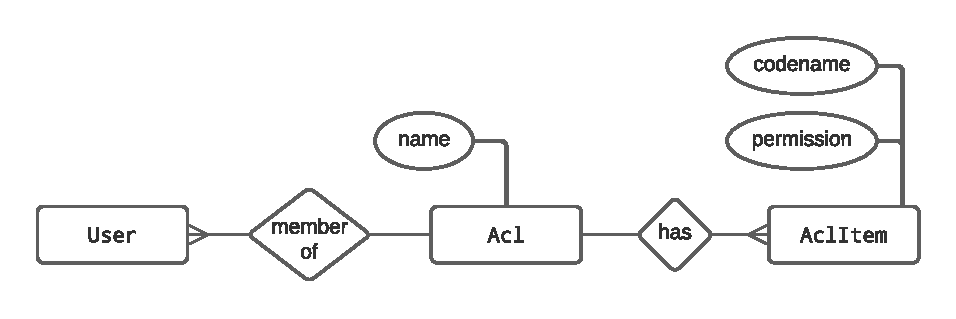
\includegraphics[width=0.75\paperwidth]{Gambar/erd-details/ERD--New - ACL & ACLItem.pdf}
        \caption{Potongan diagram entitas untuk \texttt{ACL} dan \texttt{ACLItem}.}
        \label{fig:erd_acl-aclitem}
    \end{figure}
    
    Entitas \texttt{ACL} dan \texttt{ACLItem} adalah entitas yang menampung informasi 
    tentang peran dan izin untuk
    setiap pengguna, diperjelas pada Gambar \ref{fig:erd_acl-aclitem}. 
    \texttt{ACL} menyimpan grup utama dari \texttt{ACLItem}, atau dapat kita 
    sebut sebagai peran.
    Sedangkan \texttt{ACLItem} menyimpan informasi izin untuk setiap nama 
    kasus (\texttt{codename}) yang diperbolehkan.
    
    \begin{table}[H]
        \centering
        \begin{tabular}{|l|l|l|}
        \hline
        Label & Deskripsi & Nilai Biner \\ \hline
        C     & Buat      & \texttt{0b0001}        \\ \hline
        R     & Baca      & \texttt{0b0010}        \\ \hline
        U     & Perbarui  & \texttt{0b0100}        \\ \hline
        D     & Hapus     & \texttt{0b1000}        \\ \hline
        \end{tabular}
        \caption{Tabel representasi nilai biner pada kolom \texttt{permission} di entitas \texttt{ACLItem}}
        \label{tab:aclitem_level}
    \end{table}
        
    
    Perizinan direpresentasikan dengan menggunakan sistem biner yang disimpan pada database sebagai angka.
    Representasi biner ini terdiri dari label CRUD, dengan C adalah Buat (\textit{Create}), R adalah
    Baca (\textit{Read}), U adalah Perbaharui (\textit{Update}) dan D adalah Hapus (\textit{Delete}).
    Label tersebut kemudian diberikan tempat khusus pada bitstring sebelum akhirnya dikonversi
    sebagai angka. Nilai-nilai tersebut dapat dilihat pada tabel \ref{tab:aclitem_level}.
    
    
    Sebagai contoh, seorang pengguna dapat \textbf{membuat}, \textbf{membaca}, \textbf{memperbarui}
    namun tidak dapat menghapus sebuah entri. Nilai dari tabel \ref{tab:aclitem_level} digabungkan
    dengan operator \texttt{OR} untuk setiap izin yang diberikan.
    Dengan begitu, nilai \texttt{permission} yang diberikan adalah sebagai berikut:
    
    \begin{subequations}
        \begin{align}
            C \vee R \vee U \vee 0b0000 &= K\\
            0b0001 \vee 0b0010 \vee 0b0100 \vee 0b0000 &= K \\
            K &= 0b0111 \\
            K &= 7
        \end{align}
    \end{subequations}
    
    Hasil kalkulasi kode izin tersebut akan disimpan sebagai 7 pada database sebagai representasi
    kode izin \texttt{0b000}. 
    
    Pengecekan izin \texttt{permission} dilakukan dengan memanfaatkan operator \texttt{AND} antara 
    nilai pada kolom \texttt{permission} dengan nilai \texttt{permission} yang diekspektasikan, lalu
    dibandingkan dengan nilai ekspektasi.
    Sebagai contoh, sistem perlu mengecek apakah pengguna dapat membuat sebuah entri. 
    Sistem dapat melakukan pengecekkan dengan melakukan operasi \texttt{AND} pada nilai 
    \texttt{permission} yang ada saat ini (\texttt{0111}) dengan nilai \texttt{permission} yang
    diekspektasi (\texttt{0010}), dan hasilnya dibandingkan dengan hasil ekspektasi. Kalkulasi
    yang dilakukan dapat dilihat pada simulasi ekuasi berikut:
    
    \begin{subequations}
        \begin{align}
            K \wedge C &= C \\
            0b0111 \wedge C &= C \\
            0b0111 \wedge 0b0001 &= 0b0001 \\
            0b0001 &= 0b0001 \\
            \text{True}
        \end{align}
    \end{subequations}
    
    Sedangkan jika pengecekan apakah seorang pengguna dapat melakukan penghapusan terhadap sebuah entri,
    perhitungan perizinannya menjadi:
    
    \begin{subequations}
        \begin{align}
            K \wedge D &= D \\
            0b0111 \wedge D &= D \\
            0b0111 \wedge 0b1000 &= 0b1000 \\
            0b0000 &= 0b1000 \\
            \text{False}
        \end{align}
    \end{subequations}
    
    Hasil dari ekuasi tersebut kemudian dapat digunakan untuk menentukan apakah seorang pengguna dapat
    melakukan aksi yang diminta atau tidak.
    
    Operasi ini terinspirasi dari \texttt{chmod} dari Linux\footnote{Lihat https://linux.die.net/man/1/chmod}.
    \texttt{chmod} menerima input berupa tiga angka yang merepresentasikan level akses pada \textit{resource}
    tertentu pada sistem. Tiga angka tersebut kemudian diubah menjadi biner untuk dilihat apakah
    seorang pengguna dapat melakukan aksi tertentu. Pendekatan ini kemudian diadaptasi pada sistem ini
    dengan menggunakan level akses yang berbeda (CRUD, dibanding RWX). Dengan begitu pengaturan dan
    pengelolaan resources pada entitas dapat lebih terkontrol dengan lebih fleksibel.
    
\subsubsection{IPLogin}
    \begin{figure}
        \centering
        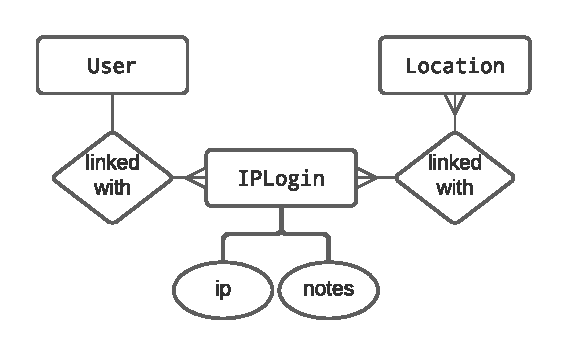
\includegraphics{Gambar/erd-details/ERD--New - IPLogin.pdf}
        \caption{Potongan diagram entitas untuk \texttt{IPLogin}.}
        \label{fig:erd_iplogin}
    \end{figure}
    Entitas \texttt{IPLogin} digunakan untuk melakukan otentikasi semi-otomatis dengan memanfaatkan IP
    pengguna pada lab, ditautkan dengan sebuah akun pengguna dengan peran yang terbatas (hanya
    dapat melihat dan mengubah entitas tertentu), diperjelas pada Gambar \ref{fig:erd_iplogin}.
    Entitas menyimpan informasi IP, tautan pada pengguna dan lokasi-lokasi, serta catatan khusus
    tentang penautan tersebut. 
    
    Entitas ini memiliki hubungan \textit{many-to-many} dengan entitas \texttt{Location}. Relasi
    ini diharapkan agar Tim Admin dapat melakukan pengaturan komputer master untuk melihat 
    seluruh ujian yang aktif pada ruangan tertentu tanpa harus membuatkan akun khusus 
    tertentu pada sistem. Tim Admin dapat dengan mudah menautkan sejumlah ruangan yang diinginkan
    dengan akun yang memiliki peranan terbatas yang sudah ada sebelumnya.
    
    Entitas ini dinilai cukup esensial karena berhubungan dengan sistem otentikasi yang membatasi
    pengguna untuk melakukan aksi tertentu di admin panel.
    
\subsubsection{Location dan Computer}
    \begin{figure}
        \centering
        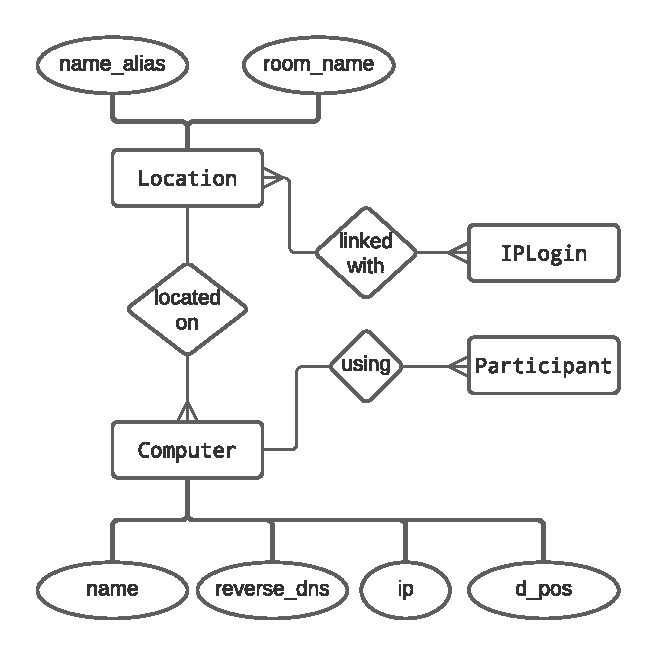
\includegraphics{Gambar/erd-details/ERD--New - Location & Computer.pdf}
        \caption{Potongan diagram entitas untuk \texttt{Location} dan \texttt{Computer}.}
        \label{fig:erd_location-computer}
    \end{figure}
    
    Entitas \texttt{Location} dan \texttt{Computer} menyimpan informasi tentang lokasi (ruagan) dan
    daftar pada komputer tersebut sebelum nantinya dihubungkan dengan entitas lainnya. Hubungan
    antara kedua entitas tersebut dapat diperhatikan pada potongan diagram entitas di gambar
    \ref{fig:erd_location-computer}.
    
    Entitas \texttt{Location} menyimpan informasi lokasi dan ruangan tempat peserta dapat mengikuti
    ujian. Pada entitas ini, informasi yang disimpan adalah nama ruangan tersebut dan nama lain
    dari ruangan tersebut. Berdasarkan survei lapangan, setiap ruangan memiliki nama lain, sehingga
    kolom \texttt{name\_alias} ditambahkan. Sedangkan nama ruangan disimpan pada kolom \texttt{room\_name}.
    
    Entitas \texttt{Computer} mendefinisikan komputer yang terdapat pada lokasi tersebut. Oleh karena
    itu hubungan yang dimiliki dengan entitas \texttt{Location} adalah \textit{one-to-many}.
    Entitas ini menyimpan informasi berupa nama komputer (\textit{name}), IPnya (\textit{ip}),
    nama FQDN (\textit{Fully Qualified Domain Name}) atau domain dari komputer tersebut (\textit{reverse\_dns}),
    dan detil letak posisi dari komputer tersebut pada peta ruangan (\textit{d\_pos}).
    
    Kolom \textit{d\_pos} digunakan untuk menyimpan informasi letak komputer pada peta dalam bentuk
    JSON. Bentuk format ini digunakan karena data ini digunakan hanya pada sistem frontend. Dengan
    kesepakatan yang diharapkan cukup fleksibel, maka bentuk pemosisian ini akan disimpan dalam 
    bentuk JSON.
    
    Kolom \textit{ip} digunakan untuk menautkan sebuah komputer dengan IP, sehingga tabel otentikasi
    yang digunakan oleh peserta dapat langsung merujuk pada entitas ini. Setiap komputer peserta
    yang ingin digunakan akan didaftarkan pada entitas ini. Untuk saat ini, karena survei lapangan
    menunjukan bahwa versi IP yang digunakan adalah versi 4, maka fokus aplikasi saat ini akan
    menggunakan IPv4.
    
    Selain itu, terdapat kolom \textit{reverse\_dns} yang digunakan untuk menyimpan informasi nama domain dari
    komputer tersebut. Kolom ini diharapkan dapat membantu Tim Admin dan pengembang aplikasi
    berikutnya untuk melakukan \textit{debugging} dan kebutuhan API lainnya. Nama domain ini didapatkan dari
    LDAP yang digunakan oleh Server Windows untuk melakukan auditing objek mereka. Komputer yang
    terhubung dengan Active Directory milik Lab akan terdaftar pada sistem internal LDAP milik Windows
    Server yang nantinya akan diberikan domain khusus untuk komputer tersebut.

\subsubsection{Lecture dan LecturePeriod}

    \begin{figure}
        \centering
        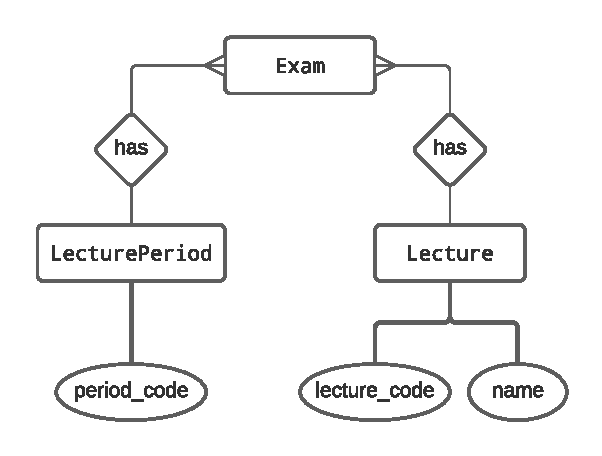
\includegraphics{Gambar/erd-details/ERD--New - Lecture & LecturePeriod.pdf}
        \caption{Potongan diagram entitas untuk \texttt{Lecture} dan \texttt{LecturePeriod}}
        \label{fig:erd_lecture-lectureperiod}
    \end{figure}

    Entitas \texttt{Lecture} dan \texttt{LecturePeriod} menyimpan informasi tentang mata kuliah
    dan periode tahun ajar mata kuliah bersangkutan pada ujian tertentu. Hubungan antara kedua
    entitas tersebut terhadap entitas \texttt{Exam} dapat dilihat pada potongan diagram entitas di 
    gambar \ref{fig:erd_lecture-lectureperiod}.  Entitas \texttt{Lecture} menyimpan informasi nama
    mata kuliah beserta kodenya, dan \texttt{LecturePeriod} menyimpan informasi tahun ajaran
    dalam bentuk kode.
    
    \begin{table}[]
        \centering
        \begin{tabular}{|l|l|}
        \hline
        Nilai & Tipe Semester \\ \hline
        1     & Ganjil        \\ \hline
        2     & Genap         \\ \hline
        3     & Pendek        \\ \hline
        \end{tabular}
        \caption{Definisi tipe semester dengan nilainya untuk kolom
            \texttt{period\_code} pada entitas \texttt{LecturePeriod}}
        \label{tab:lecture-periode}
    \end{table}
    
    Kode tersebut terdiri dari lima digit angka yang terdiri dari tahun ajar dan tipe semester
    yang sedang berjalan. Empat digit pertama adalah tahun ajar, dan satu digit terakhir adalah
    tipe semester. Tipe semester dan nilai representasinya dapat dilihat lebih jelas pada tabel
    \ref{tab:lecture-periode}.
    
    Sebagai contoh, semester ganjil pada tahun ajar 2016-2017 direpresentasikan sebagai
    \texttt{20161}. Empat digit pertama diambil dari tahun ajar pada tahun dimulai, 2016. Lalu
    berdasarkan tabel \ref{tab:lecture-periode}, semester ganjil memiliki nilai representasi
    1, sehingga kode untuk tahun ajar yang disimpan pada kolom \textit{period\_code} 
    adalah \texttt{20161}.
    
\subsubsection{Participant}
    \begin{figure}
        \centering
        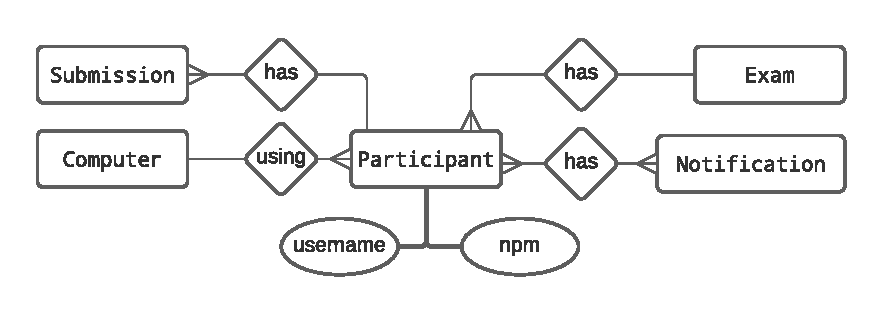
\includegraphics{Gambar/erd-details/ERD--New - Participant.pdf}
        \caption{Potongan diagram entitas untuk \texttt{Participant}}
        \label{fig:erd_participant}
    \end{figure}
    
    Entitas \texttt{Participant} digunakan untuk menyimpan informasi tentang peserta
    ujian di lab. Seperti pada potongan diagram relasi entitas pada gambar \ref{fig:erd_participant},
    entitas ini hanya memiliki dua kolom utama yang digunakan untuk merepresentasikan
    seorang peserta. Kolom \texttt{username} untuk menyimpan informasi username pada sistem
    dan \texttt{npm} untuk menyimpan informasi NPM dari peserta.
    
    Kolom \texttt{npm} digunakan untuk menyimpan string \textit{literal} dari nomor pokok mahasiswa
    (NPM). Karena NPM mahasiswa yang aktif pada saat penelitian ini dibuat terdapat dua standar, maka
    untuk memperingan kinerna basis data, string \textit{literal} NPM ikut disimpan.
    
    Sedangkan kolom \texttt{username} digunakan untuk menyimpan username yang biasa digunakan
    di lab untuk login. Kolom ini akan berguna untuk membantu sistem mebuat \textit{script batch}
    pada tahap pemberian akses ke berkas bantuan ujian dan \textit{workspace} peserta ujian. 
    Pemberian akses dengan script membutuhkan nama pengguna yang digunakan untuk login.
    
\subsubsection{AnswerSlot}
    Entitas \texttt{AnswerSlot} digunakan untuk menyimpan informasi tentang slot jawaban 
    pada ujian tertentu. Entitas ini digunakan sebagai panduan untuk sistem memberikan
    informasi tentang format penamaan file, disimpan pada kolom \texttt{format}. 
    Seperti yang terlihat pada
    diagram entitas pada \ref{fig:erd_overview}, entitas ini akan terhubung secara 
    \textit{many-to-one} terhadap entitas \texttt{exam} dan \textit{one to many} pada entitas
    \texttt{Submission}.
    
    Jawaban yang dikirimkan oleh peserta nantinya akan disimpan pada entitas \texttt{Submission}
    dengan bantuan referensi format dari \texttt{AnswerSlot}. Setiap jawaban yang dikumpulkan akan dicek
    formatnya berdasarkan format yang diberikan pada entitas \textit{AnswerSlot}.

\subsubsection{ExamReport}
    Entitas \texttt{ExamReport} digunakan untuk membantu sistem menjadwalkan pengiriman laporan
    ujian. Laporan ini nantinya direncanakan untuk dikirimkan via email untuk mengatisipasi email
    diblokir oleh penyedia layanan email karena kode Java dan berkas \texttt{.class}nya dianggap 
    sebagai virus.
    
    Seperti yang ditunjukkan pada diagram entitas pada gambar \ref{fig:erd_overview}, entitas 
    \texttt{ExamReport} menyimpan beberapa kolom yang digunakan untuk membantu penjadwalan.
    Kolom pertama adalah \texttt{sent\_on} yang digunakan untuk menandakan apakah ujian ini
    telah dikirimkan pada email (\texttt{to(s)}) ini. Kolom \texttt{valid\_until} digunakan
    untuk menyimpan informasi kapan \texttt{token} akan kadaluarsa (\textit{expired}).
    
    Penggunaan token pada kasus ini dengan harapan alamat link yang dikirim oleh sistem
    ke dosen dapat dengan aman di akses. Kode token akan terdiri dari 16 byte acak yang
    dikonversi menjadi 32 digit heksadesimal string. Token ini diharapkan 
    dibangkitkan dengan standar pengacakan untuk kriptografi.  Pengacakan dengan standar 
    tersebut diharapkan dapat memperkecil faktor kemungkinan serangan prediksi 
    kode token (\textit{guessing attack}).

\subsubsection{Exam}
    \begin{figure}
        \centering
        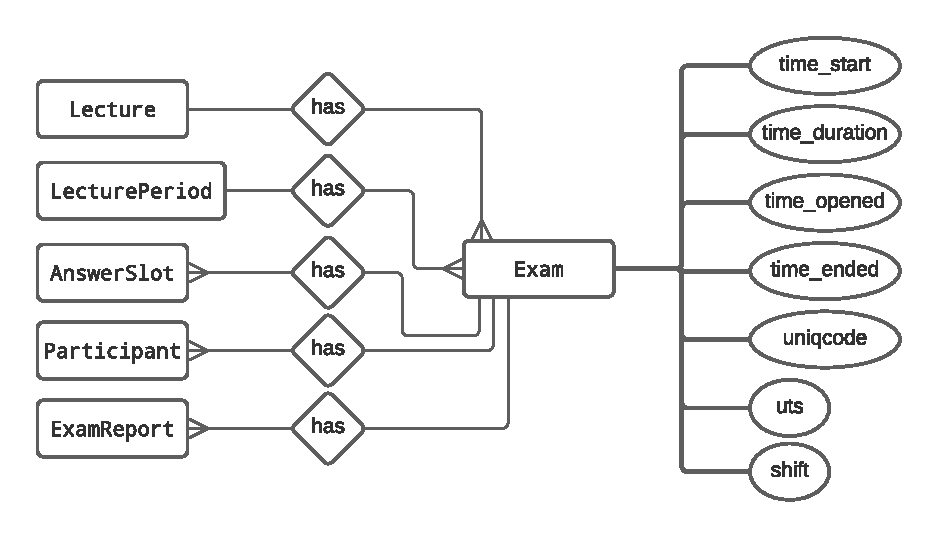
\includegraphics[width=0.75\paperwidth]{Gambar/erd-details/ERD--New - Exam.pdf}
        \caption{Potongan diagram entitas untuk \texttt{Exam}.}
        \label{fig:erd_exam}
    \end{figure}
    Entitas berikutnya yang akan dibahas adalah entitas \texttt{Exam}, dapat dilihat pada potongan
    gambar \ref{fig:erd_exam}. Entitas ini menyimpan informasi utama untuk ujian dan jadwalnya.
    Informasi jadwal disimpan pada kolom dengan \textit{prefix} \texttt{time\_}. Informasi dasar
    dari ujian tersebut disimpan dengan relasi langsung ke tabel lain seperti \texttt{Lecture},
    \texttt{LecturePeriod}, \texttt{AnswerSlot}, dan seterusnya. 
    
    Informasi yang cukup penting pada entitas ini terdapat pada kolom \texttt{uniqcode}. Kolom
    ini menyimpan informasi kode unik dari sebuah ujian yang kita gunakan untuk menyimpan informasi
    nama folder berkas ujian. Kode ini diharapkan terdiri dengan byte acak yang dibangkitkan dengan
    standar pengacakan untuk kriptografi. Pengacakan dengan standar tersebut diharapkan dapat
    memperkecil faktor kemungkinan serangan prediksi kode unik (\textit{guessing attack}).
    
    Pengecekan ujian yang aktif dilakukan dengan melakukan pengecekan pada kolom 
    \texttt{time\_start} dan \texttt{time\_ended}. Kolom \texttt{time\_start} menandakan
    informasi tentang kapan ujian \textbf{akan} dimulai. Kolom ini tidak menentukan kapan
    lembar jawaban dapat di\textit{submit} oleh peserta ujian. Sedangkan kolom \texttt{time\_ended}
    menandakan informasi tentang kapan lembar jawaban ditutup.
    
    Untuk membuka lembar jawaban, kolom \texttt{time\_opened} dan \texttt{time\_ended} harus diisi
    dengan informasi tanggal kapan lembar jawaban telah dibuka. Pada keadaan bawaan, normalnya
    kolom-kolom tersebut seharusnya memiliki nilai \texttt{NULL}. Pada saat Dosen Pengawas melakukan
    aksi membuka jawaban, maka kedua kolom tersebut harus diisi sesuai dengan durasi yang diberikan
    pada kolom \texttt{time\_duration}. Pengisian kolom \texttt{time\_opened} dam \texttt{time\_ended}
    diharapkan dapat mengurangi beban sistem untuk melakukan perhitungan secara terus menerus jika
    \texttt{time\_ended} tidak diberikan. Selain itu, dengan mengisi dua kolom tersebut secara
    simultan, diharapkan dapat mengurangi potensi masalah ujian lupa ditutup.
    
\subsubsection{Submission}
    
    \begin{figure}[H]
        \centering
        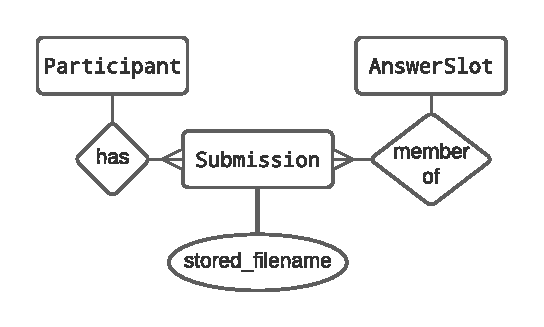
\includegraphics{Gambar/erd-details/ERD--New - Submission.pdf}
        \caption{Potongan diagram relasi entitas untuk \texttt{Submission}}
        \label{fig:erd_submission}
    \end{figure}

    Entitas \texttt{Submission}, seperti yang dapat dilihat pada potongan diagram relasi entitas 
    \ref{fig:erd_submission}, menampung informasi tentang submisi yang dilakukan oleh
    peserta ujian. Submisi yang dikirimkan direncanakan untuk disimpan dengan nama berkas
    yang acak. Nama berkas tersebut kemudian disimpan pada database sebagai referensi untuk nantinya
    pelaporan yang dibantu oleh entitas \texttt{ExamReport}.
    
    Submisi yang dikirimkan oleh peserta akan dicek formatnya dengan bantuan dari entitas 
    \texttt{AnswerSlot}. Jika nama berkas sudah sesuai dengan format, maka data akan dimasukan
    pada entitas ini.
    
\subsubsection{Notification}
    Entitas \texttt{Notification} menyimpan informasi tentang notifikasi yang diberikan
    pada peserta. Karena beragam notifikasi dapat diberikan pada peserta, seperti informasi tentang
    kredensial untuk masuk ke sistem judge atau basis data; atau informasi tentang ralat soal.
    Oleh karena itu hubungan yang dimiliki entitas ini dengan entitas peserta adalah
    \textit{many-to-many}.
    
    Seperti pada diagram relasi entitas pada gambar \ref{fig:erd_overview}, entitas 
    \texttt{Notification} memiliki beberapa kolom untuk menyimpan isi notifikasi 
    (\texttt{description}) dan judul (\texttt{title}). Kolom lainnya, seperti \texttt{type} digunakan
    untuk memasukan notifikasi terhadap grup tertentu. Kolom yang terakhir adalah 
    kolom \texttt{extras}. Semua informasi yang tidak dapat direpresentasikan pada kolom akan
    disimpan dalam bentuk JSON pada kolom ini. Kolom ini disediakan karna kebutuhan fleksibilitas
    notifikasi yang mungkin akan muncul di masa yang akan datang.

\subsection{Rancangan REST API}
    REST API dirancang dengan pola yang seragam pada beberapa \textit{endpoint} besar, sehingga
    penggunaan API dapat lebih optimal diaplikasikan dengan metode abstraksi API class pada sistem
    frontend.
    
    Perancangan REST API dimulai dengan merencanakan metode otentikasi yang akan digunakan untuk
    setiap permintaan. Lalu pembahsan dilanjutkan dengan desain URL yang digunakan dan tujuannya.
    
    % sistem otentikasi
\subsubsection{Otentikasi API}
    Sesuai dengan kebutuhan, Otentikasi API terbagi menjadi dua bagian besar berdasarkan penggunaannya.
    Otentikasi API yang pertama dilakukan dengan menggunakan IP, sedangkan yang kedua, otentikasi
    dilakukan dengan menggunakan token.
    %TODO: MORE
    
    Otentikasi dengan IP diperuntukkan untuk API yang berhubungan dengan ujian pada lokasi yang telah
    didefinisikan sebelumnya. IP digunakan karena sistem sebelumnya menggunakan cara ini dan telah
    terbukti di "medan perang" bahwa cara ini sudah sangat efektif. Pengguna tidak perlu melakukan
    otentikasi secara manual dengan memasukkan kredensial khusus untuk sistem. Otentikasi dengan IP
    juga tidak memaksa klien untuk melakukan refresh secara terus menerus untuk memperbarui 
    \textit{session} mereka, seperti pada aplikasi sebelumnya.
    
    Otentikasi dengan token dilakukan dengan melakukan otentikasi manual hingga sistem memberikan
    sebuah string khusus yang digunakan sebagai token untuk setiap permintaan. Otentikasi
    manual tersebut dapat berupa memasukan kredensial login, atau dengan token khusus yang sebelumnya
    diberikan pada email. Token ini nantinya dapat digunakan untuk mengakses berbagai 
    \textit{resources} yang backend sediakan. Seperti tombol unduh pada halaman laporan, atau
    melakukan CRUD pada entitas tertentu.
    Token yang digunakan pada sistem normalnya akan menggunakan JSON Web Token atau JWT, dengan bantuan 
    \textit{library} dari backend. Rencananya JWT ini akan menggunakan algoritma kunci asimetrik,
    sebagai standar keamanan.
    
    % desail url berdasarkan rest API
\subsubsection{Desain \textit{Endpoint}}
    Dengan beragam kebutuhan yang muncul, design URL untuk REST API juga harus mengikuti. REST API
    yang ada akan 
    
    % Bagian Otentiksi
\subsubsection{Desain \textit{Endpoint} Otentikasi}

    % Bagian Exam
\subsubsection{Desain \textit{Endpoint} Ujian}
    
    % Bagian Admin
\subsubsection{Desain \textit{Endpoint} Admin}
    
    % Bagian Dosen
\subsubsection{Desain \textit{Endpoint} Lainnya}
    
\subsection{Desain Kelas}
    % diagram kelas
    
\section{Perancangan Sistem Frontend}
    % diagram kelas dan file
    
    % Jelasin komponennya satu satu
\section{Perancangan Sistem CI/CD dan Unit Testing}
    
    % melakukan build pada saat commit
    
    
    % melakukan unit testing pada saat commit
    % unit testing yang dilakukan cuma buat 